\documentclass[14pt]{extarticle}
\usepackage[letterpaper, left=0.75in, right=0.75in, top=0.85in, bottom=0.85in, headsep=0.25in, footskip=0.4in]{geometry}
\usepackage[T1]{fontenc}
\usepackage[scaled=0.95]{helvet}
\renewcommand{\familydefault}{\sfdefault}
\usepackage{tikz}
\usetikzlibrary{arrows.meta}
\usepackage{fancyhdr}
\pagestyle{fancy}
\fancyhf{}
\renewcommand{\headrulewidth}{0pt}
\lhead{\small Week NN / Pancake flips / Grades K--1}
\lfoot{\small Bellingham Math Circle / Week NN / NN-K-v1}
\rfoot{\small \thepage}
\setlength{\parindent}{0pt}
\setlength{\parskip}{6pt}
\definecolor{cakefillc}{RGB}{248,224,170}
\definecolor{cakedrawc}{RGB}{140,95,35}
\definecolor{burntc}{RGB}{85,50,20}
\tikzset{
  cakefill/.style={fill=cakefillc},
  cakedraw/.style={draw=cakedrawc, line width=0.9pt},
  burnt/.style={fill=burntc},
  platedraw/.style={draw=black!55, line width=0.6pt},
  platefill/.style={fill=black!18},
  slot/.style={draw=black!70, dashed, line width=0.8pt},
  spatula/.style={fill=black!65},
  handle/.style={fill=black!40},
  tokdraw/.style={draw=black!70, line width=0.8pt},
  tokfill/.style={fill=black!12},
  breakmark/.style={draw=red!80!black, line width=1.8pt, line cap=round},
}
\newcommand{\problem}[1]{\par\medskip\textbf{Problem #1:}\ }
\begin{document}
A stack is sorted when it goes from the smallest pancake on top to the biggest at the bottom. To flip, slide the spatula under a pancake and turn over everything above the spatula, all together. Put down a token for each flip.
\par\smallskip\begin{center}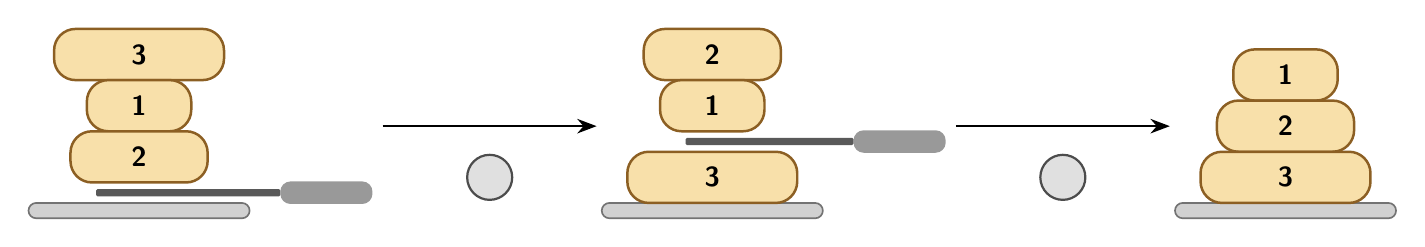
\begin{tikzpicture}
\draw[platedraw, platefill, rounded corners=0.098cm] (-1.404,-0.195) rectangle (1.404,0);
\fill[cakefill] [rounded corners=0.273cm] (-1.079,1.560) rectangle (1.079,2.210);
\draw[cakedraw] [rounded corners=0.273cm] (-1.079,1.560) rectangle (1.079,2.210);
\node[font=\normalsize\bfseries, inner sep=0pt] at (0.000,1.885) {3};
\fill[cakefill] [rounded corners=0.273cm] (-0.663,0.910) rectangle (0.663,1.560);
\draw[cakedraw] [rounded corners=0.273cm] (-0.663,0.910) rectangle (0.663,1.560);
\node[font=\normalsize\bfseries, inner sep=0pt] at (0.000,1.235) {1};
\fill[cakefill] [rounded corners=0.273cm] (-0.871,0.260) rectangle (0.871,0.910);
\draw[cakedraw] [rounded corners=0.273cm] (-0.871,0.260) rectangle (0.871,0.910);
\node[font=\normalsize\bfseries, inner sep=0pt] at (0.000,0.585) {2};
\fill[spatula, rounded corners=0.5pt] (-0.546,0.084) rectangle (1.794,0.176);
\fill[handle, rounded corners=0.129cm] (1.794,-0.013) rectangle (2.964,0.273);
\draw[-{Stealth[length=7pt]}, thick] (3.094,0.975) -- (5.811,0.975);
\draw[tokdraw, tokfill] (4.453,0.325) circle (0.286);
\draw[platedraw, platefill, rounded corners=0.098cm] (5.876,-0.195) rectangle (8.684,0);
\fill[cakefill] [rounded corners=0.273cm] (6.409,1.560) rectangle (8.151,2.210);
\draw[cakedraw] [rounded corners=0.273cm] (6.409,1.560) rectangle (8.151,2.210);
\node[font=\normalsize\bfseries, inner sep=0pt] at (7.280,1.885) {2};
\fill[cakefill] [rounded corners=0.273cm] (6.617,0.910) rectangle (7.943,1.560);
\draw[cakedraw] [rounded corners=0.273cm] (6.617,0.910) rectangle (7.943,1.560);
\node[font=\normalsize\bfseries, inner sep=0pt] at (7.280,1.235) {1};
\fill[cakefill] [rounded corners=0.273cm] (6.201,0.000) rectangle (8.359,0.650);
\draw[cakedraw] [rounded corners=0.273cm] (6.201,0.000) rectangle (8.359,0.650);
\node[font=\normalsize\bfseries, inner sep=0pt] at (7.280,0.325) {3};
\fill[spatula, rounded corners=0.5pt] (6.942,0.735) rectangle (9.074,0.826);
\fill[handle, rounded corners=0.129cm] (9.074,0.637) rectangle (10.244,0.923);
\draw[-{Stealth[length=7pt]}, thick] (10.374,0.975) -- (13.091,0.975);
\draw[tokdraw, tokfill] (11.732,0.325) circle (0.286);
\draw[platedraw, platefill, rounded corners=0.098cm] (13.156,-0.195) rectangle (15.964,0);
\fill[cakefill] [rounded corners=0.273cm] (13.897,1.300) rectangle (15.223,1.950);
\draw[cakedraw] [rounded corners=0.273cm] (13.897,1.300) rectangle (15.223,1.950);
\node[font=\normalsize\bfseries, inner sep=0pt] at (14.560,1.625) {1};
\fill[cakefill] [rounded corners=0.273cm] (13.689,0.650) rectangle (15.431,1.300);
\draw[cakedraw] [rounded corners=0.273cm] (13.689,0.650) rectangle (15.431,1.300);
\node[font=\normalsize\bfseries, inner sep=0pt] at (14.560,0.975) {2};
\fill[cakefill] [rounded corners=0.273cm] (13.481,0.000) rectangle (15.639,0.650);
\draw[cakedraw] [rounded corners=0.273cm] (13.481,0.000) rectangle (15.639,0.650);
\node[font=\normalsize\bfseries, inner sep=0pt] at (14.560,0.325) {3};
\end{tikzpicture}\end{center}
\problem{1}Find all six ways to stack pancakes 1, 2 and 3, and sort each one with as few flips as you can. Circle the stack that needs the most flips.
\par\medskip
\noindent\makebox[\linewidth][s]{\hfill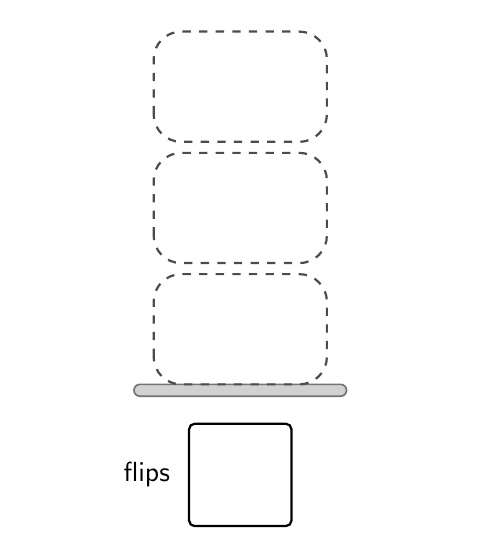
\begin{tikzpicture}
\useasboundingbox (-2.700,-1.850) rectangle (2.700,4.530);
\draw[platedraw, platefill, rounded corners=0.075cm] (-1.350,-0.150) rectangle (1.350,0);
\draw[slot, rounded corners=0.350cm] (-1.100,3.080) rectangle (1.100,4.480);
\draw[slot, rounded corners=0.350cm] (-1.100,1.540) rectangle (1.100,2.940);
\draw[slot, rounded corners=0.350cm] (-1.100,0.000) rectangle (1.100,1.400);
\node[anchor=east, font=\normalsize] at (-0.770,-1.150) {flips};
\draw[thick, rounded corners=2pt] (-0.650,-1.800) rectangle (0.650,-0.500);
\end{tikzpicture}\hfill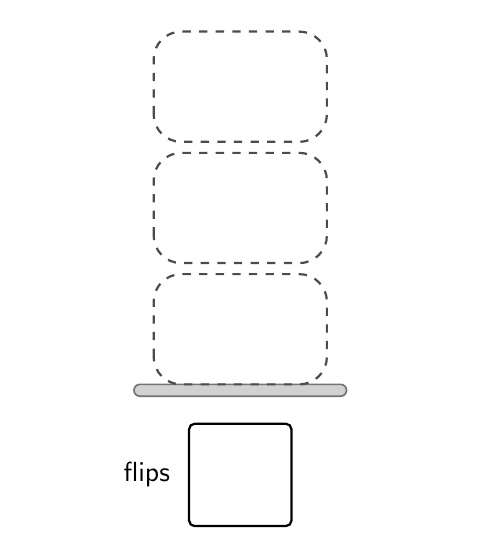
\begin{tikzpicture}
\useasboundingbox (-2.700,-1.850) rectangle (2.700,4.530);
\draw[platedraw, platefill, rounded corners=0.075cm] (-1.350,-0.150) rectangle (1.350,0);
\draw[slot, rounded corners=0.350cm] (-1.100,3.080) rectangle (1.100,4.480);
\draw[slot, rounded corners=0.350cm] (-1.100,1.540) rectangle (1.100,2.940);
\draw[slot, rounded corners=0.350cm] (-1.100,0.000) rectangle (1.100,1.400);
\node[anchor=east, font=\normalsize] at (-0.770,-1.150) {flips};
\draw[thick, rounded corners=2pt] (-0.650,-1.800) rectangle (0.650,-0.500);
\end{tikzpicture}\hfill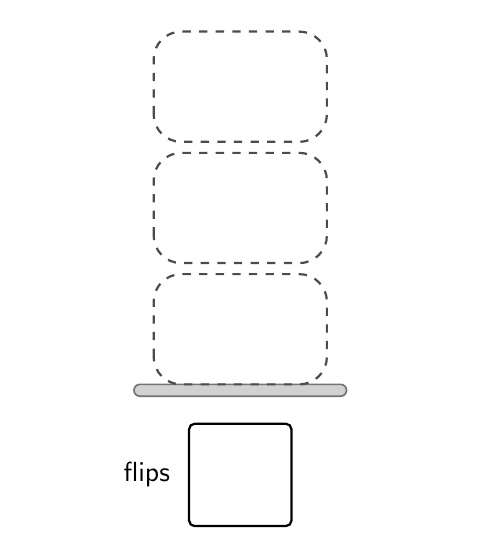
\begin{tikzpicture}
\useasboundingbox (-2.700,-1.850) rectangle (2.700,4.530);
\draw[platedraw, platefill, rounded corners=0.075cm] (-1.350,-0.150) rectangle (1.350,0);
\draw[slot, rounded corners=0.350cm] (-1.100,3.080) rectangle (1.100,4.480);
\draw[slot, rounded corners=0.350cm] (-1.100,1.540) rectangle (1.100,2.940);
\draw[slot, rounded corners=0.350cm] (-1.100,0.000) rectangle (1.100,1.400);
\node[anchor=east, font=\normalsize] at (-0.770,-1.150) {flips};
\draw[thick, rounded corners=2pt] (-0.650,-1.800) rectangle (0.650,-0.500);
\end{tikzpicture}\hfill}

\par\vspace{0.9cm}
\noindent\makebox[\linewidth][s]{\hfill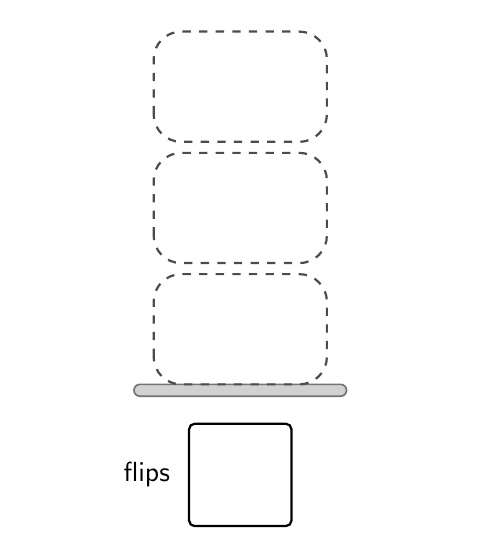
\begin{tikzpicture}
\useasboundingbox (-2.700,-1.850) rectangle (2.700,4.530);
\draw[platedraw, platefill, rounded corners=0.075cm] (-1.350,-0.150) rectangle (1.350,0);
\draw[slot, rounded corners=0.350cm] (-1.100,3.080) rectangle (1.100,4.480);
\draw[slot, rounded corners=0.350cm] (-1.100,1.540) rectangle (1.100,2.940);
\draw[slot, rounded corners=0.350cm] (-1.100,0.000) rectangle (1.100,1.400);
\node[anchor=east, font=\normalsize] at (-0.770,-1.150) {flips};
\draw[thick, rounded corners=2pt] (-0.650,-1.800) rectangle (0.650,-0.500);
\end{tikzpicture}\hfill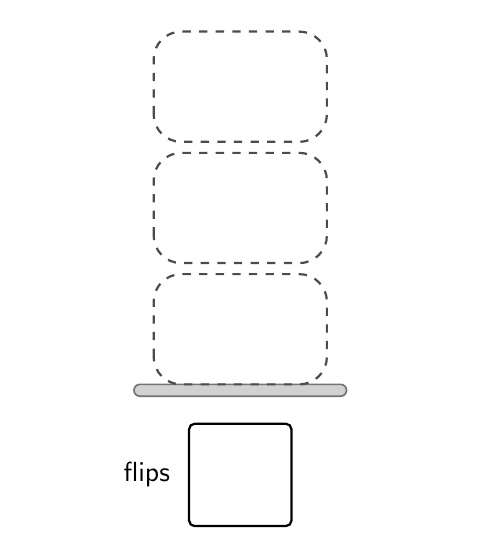
\begin{tikzpicture}
\useasboundingbox (-2.700,-1.850) rectangle (2.700,4.530);
\draw[platedraw, platefill, rounded corners=0.075cm] (-1.350,-0.150) rectangle (1.350,0);
\draw[slot, rounded corners=0.350cm] (-1.100,3.080) rectangle (1.100,4.480);
\draw[slot, rounded corners=0.350cm] (-1.100,1.540) rectangle (1.100,2.940);
\draw[slot, rounded corners=0.350cm] (-1.100,0.000) rectangle (1.100,1.400);
\node[anchor=east, font=\normalsize] at (-0.770,-1.150) {flips};
\draw[thick, rounded corners=2pt] (-0.650,-1.800) rectangle (0.650,-0.500);
\end{tikzpicture}\hfill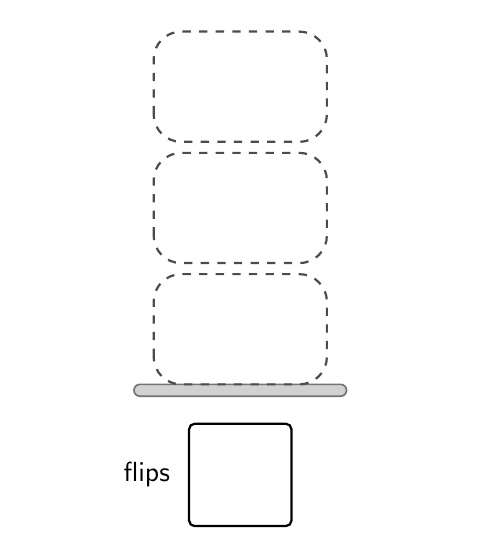
\begin{tikzpicture}
\useasboundingbox (-2.700,-1.850) rectangle (2.700,4.530);
\draw[platedraw, platefill, rounded corners=0.075cm] (-1.350,-0.150) rectangle (1.350,0);
\draw[slot, rounded corners=0.350cm] (-1.100,3.080) rectangle (1.100,4.480);
\draw[slot, rounded corners=0.350cm] (-1.100,1.540) rectangle (1.100,2.940);
\draw[slot, rounded corners=0.350cm] (-1.100,0.000) rectangle (1.100,1.400);
\node[anchor=east, font=\normalsize] at (-0.770,-1.150) {flips};
\draw[thick, rounded corners=2pt] (-0.650,-1.800) rectangle (0.650,-0.500);
\end{tikzpicture}\hfill}

\newpage
\problem{2}Build each stack of four and sort it with as few flips as you can.
\par\bigskip
\noindent\makebox[\linewidth][s]{\hfill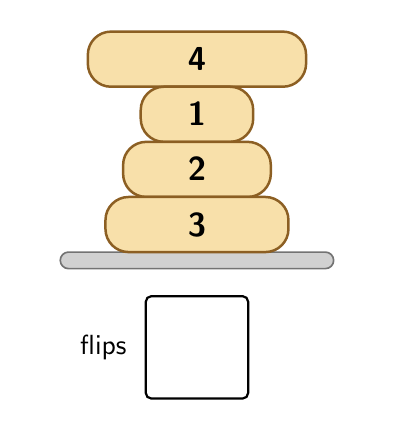
\begin{tikzpicture}
\useasboundingbox (-2.150,-1.910) rectangle (2.150,2.850);
\draw[platedraw, platefill, rounded corners=0.105cm] (-1.736,-0.210) rectangle (1.736,0);
\fill[cakefill] [rounded corners=0.294cm] (-1.386,2.100) rectangle (1.386,2.800);
\draw[cakedraw] [rounded corners=0.294cm] (-1.386,2.100) rectangle (1.386,2.800);
\node[font=\large\bfseries, inner sep=0pt] at (0.000,2.450) {4};
\fill[cakefill] [rounded corners=0.294cm] (-0.714,1.400) rectangle (0.714,2.100);
\draw[cakedraw] [rounded corners=0.294cm] (-0.714,1.400) rectangle (0.714,2.100);
\node[font=\large\bfseries, inner sep=0pt] at (0.000,1.750) {1};
\fill[cakefill] [rounded corners=0.294cm] (-0.938,0.700) rectangle (0.938,1.400);
\draw[cakedraw] [rounded corners=0.294cm] (-0.938,0.700) rectangle (0.938,1.400);
\node[font=\large\bfseries, inner sep=0pt] at (0.000,1.050) {2};
\fill[cakefill] [rounded corners=0.294cm] (-1.162,0.000) rectangle (1.162,0.700);
\draw[cakedraw] [rounded corners=0.294cm] (-1.162,0.000) rectangle (1.162,0.700);
\node[font=\large\bfseries, inner sep=0pt] at (0.000,0.350) {3};
\node[anchor=east, font=\normalsize] at (-0.770,-1.210) {flips};
\draw[thick, rounded corners=2pt] (-0.650,-1.860) rectangle (0.650,-0.560);
\end{tikzpicture}\hfill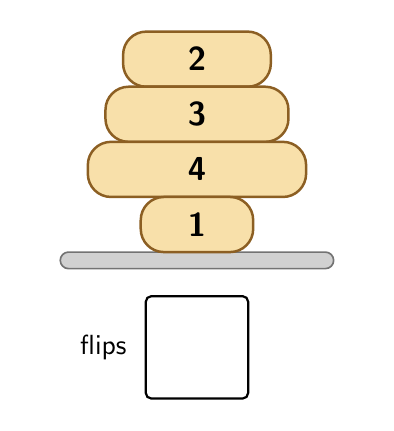
\begin{tikzpicture}
\useasboundingbox (-2.150,-1.910) rectangle (2.150,2.850);
\draw[platedraw, platefill, rounded corners=0.105cm] (-1.736,-0.210) rectangle (1.736,0);
\fill[cakefill] [rounded corners=0.294cm] (-0.938,2.100) rectangle (0.938,2.800);
\draw[cakedraw] [rounded corners=0.294cm] (-0.938,2.100) rectangle (0.938,2.800);
\node[font=\large\bfseries, inner sep=0pt] at (0.000,2.450) {2};
\fill[cakefill] [rounded corners=0.294cm] (-1.162,1.400) rectangle (1.162,2.100);
\draw[cakedraw] [rounded corners=0.294cm] (-1.162,1.400) rectangle (1.162,2.100);
\node[font=\large\bfseries, inner sep=0pt] at (0.000,1.750) {3};
\fill[cakefill] [rounded corners=0.294cm] (-1.386,0.700) rectangle (1.386,1.400);
\draw[cakedraw] [rounded corners=0.294cm] (-1.386,0.700) rectangle (1.386,1.400);
\node[font=\large\bfseries, inner sep=0pt] at (0.000,1.050) {4};
\fill[cakefill] [rounded corners=0.294cm] (-0.714,0.000) rectangle (0.714,0.700);
\draw[cakedraw] [rounded corners=0.294cm] (-0.714,0.000) rectangle (0.714,0.700);
\node[font=\large\bfseries, inner sep=0pt] at (0.000,0.350) {1};
\node[anchor=east, font=\normalsize] at (-0.770,-1.210) {flips};
\draw[thick, rounded corners=2pt] (-0.650,-1.860) rectangle (0.650,-0.560);
\end{tikzpicture}\hfill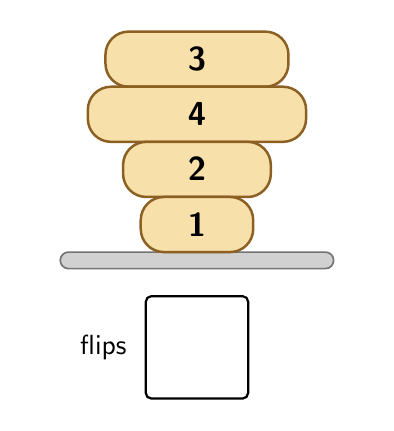
\begin{tikzpicture}
\useasboundingbox (-2.150,-1.910) rectangle (2.150,2.850);
\draw[platedraw, platefill, rounded corners=0.105cm] (-1.736,-0.210) rectangle (1.736,0);
\fill[cakefill] [rounded corners=0.294cm] (-1.162,2.100) rectangle (1.162,2.800);
\draw[cakedraw] [rounded corners=0.294cm] (-1.162,2.100) rectangle (1.162,2.800);
\node[font=\large\bfseries, inner sep=0pt] at (0.000,2.450) {3};
\fill[cakefill] [rounded corners=0.294cm] (-1.386,1.400) rectangle (1.386,2.100);
\draw[cakedraw] [rounded corners=0.294cm] (-1.386,1.400) rectangle (1.386,2.100);
\node[font=\large\bfseries, inner sep=0pt] at (0.000,1.750) {4};
\fill[cakefill] [rounded corners=0.294cm] (-0.938,0.700) rectangle (0.938,1.400);
\draw[cakedraw] [rounded corners=0.294cm] (-0.938,0.700) rectangle (0.938,1.400);
\node[font=\large\bfseries, inner sep=0pt] at (0.000,1.050) {2};
\fill[cakefill] [rounded corners=0.294cm] (-0.714,0.000) rectangle (0.714,0.700);
\draw[cakedraw] [rounded corners=0.294cm] (-0.714,0.000) rectangle (0.714,0.700);
\node[font=\large\bfseries, inner sep=0pt] at (0.000,0.350) {1};
\node[anchor=east, font=\normalsize] at (-0.770,-1.210) {flips};
\draw[thick, rounded corners=2pt] (-0.650,-1.860) rectangle (0.650,-0.560);
\end{tikzpicture}\hfill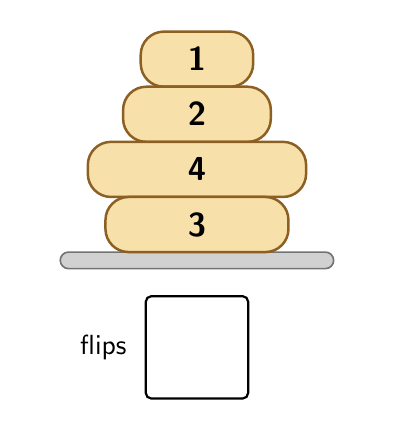
\begin{tikzpicture}
\useasboundingbox (-2.150,-1.910) rectangle (2.150,2.850);
\draw[platedraw, platefill, rounded corners=0.105cm] (-1.736,-0.210) rectangle (1.736,0);
\fill[cakefill] [rounded corners=0.294cm] (-0.714,2.100) rectangle (0.714,2.800);
\draw[cakedraw] [rounded corners=0.294cm] (-0.714,2.100) rectangle (0.714,2.800);
\node[font=\large\bfseries, inner sep=0pt] at (0.000,2.450) {1};
\fill[cakefill] [rounded corners=0.294cm] (-0.938,1.400) rectangle (0.938,2.100);
\draw[cakedraw] [rounded corners=0.294cm] (-0.938,1.400) rectangle (0.938,2.100);
\node[font=\large\bfseries, inner sep=0pt] at (0.000,1.750) {2};
\fill[cakefill] [rounded corners=0.294cm] (-1.386,0.700) rectangle (1.386,1.400);
\draw[cakedraw] [rounded corners=0.294cm] (-1.386,0.700) rectangle (1.386,1.400);
\node[font=\large\bfseries, inner sep=0pt] at (0.000,1.050) {4};
\fill[cakefill] [rounded corners=0.294cm] (-1.162,0.000) rectangle (1.162,0.700);
\draw[cakedraw] [rounded corners=0.294cm] (-1.162,0.000) rectangle (1.162,0.700);
\node[font=\large\bfseries, inner sep=0pt] at (0.000,0.350) {3};
\node[anchor=east, font=\normalsize] at (-0.770,-1.210) {flips};
\draw[thick, rounded corners=2pt] (-0.650,-1.860) rectangle (0.650,-0.560);
\end{tikzpicture}\hfill}

\par\vspace{1.4cm}
\problem{3}Find every mixed-up stack of pancakes 1, 2, 3 and 4 that you can sort with one flip.
\par\bigskip
\noindent\makebox[\linewidth][s]{\hfill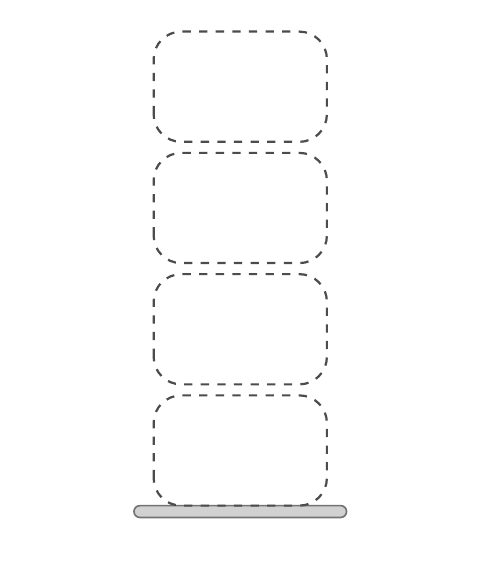
\begin{tikzpicture}
\useasboundingbox (-2.700,-0.550) rectangle (2.700,6.070);
\draw[platedraw, platefill, rounded corners=0.075cm] (-1.350,-0.150) rectangle (1.350,0);
\draw[slot, rounded corners=0.350cm] (-1.100,4.620) rectangle (1.100,6.020);
\draw[slot, rounded corners=0.350cm] (-1.100,3.080) rectangle (1.100,4.480);
\draw[slot, rounded corners=0.350cm] (-1.100,1.540) rectangle (1.100,2.940);
\draw[slot, rounded corners=0.350cm] (-1.100,0.000) rectangle (1.100,1.400);
\end{tikzpicture}\hfill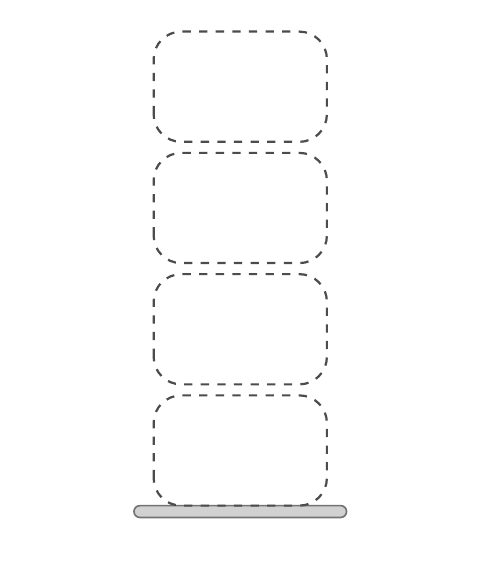
\begin{tikzpicture}
\useasboundingbox (-2.700,-0.550) rectangle (2.700,6.070);
\draw[platedraw, platefill, rounded corners=0.075cm] (-1.350,-0.150) rectangle (1.350,0);
\draw[slot, rounded corners=0.350cm] (-1.100,4.620) rectangle (1.100,6.020);
\draw[slot, rounded corners=0.350cm] (-1.100,3.080) rectangle (1.100,4.480);
\draw[slot, rounded corners=0.350cm] (-1.100,1.540) rectangle (1.100,2.940);
\draw[slot, rounded corners=0.350cm] (-1.100,0.000) rectangle (1.100,1.400);
\end{tikzpicture}\hfill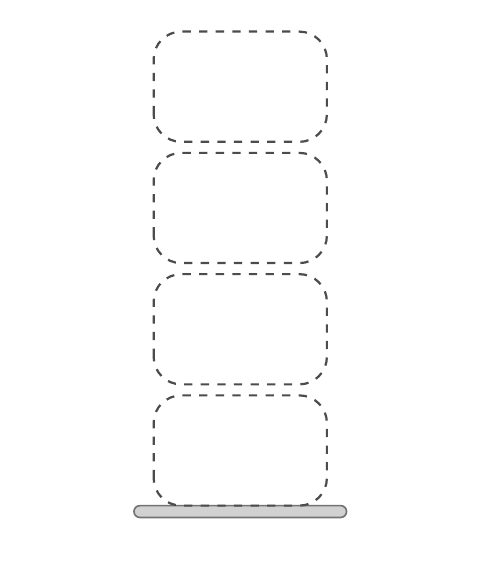
\begin{tikzpicture}
\useasboundingbox (-2.700,-0.550) rectangle (2.700,6.070);
\draw[platedraw, platefill, rounded corners=0.075cm] (-1.350,-0.150) rectangle (1.350,0);
\draw[slot, rounded corners=0.350cm] (-1.100,4.620) rectangle (1.100,6.020);
\draw[slot, rounded corners=0.350cm] (-1.100,3.080) rectangle (1.100,4.480);
\draw[slot, rounded corners=0.350cm] (-1.100,1.540) rectangle (1.100,2.940);
\draw[slot, rounded corners=0.350cm] (-1.100,0.000) rectangle (1.100,1.400);
\end{tikzpicture}\hfill}

\newpage
\problem{4}Build each stack and sort it with as few flips as you can.
\par\bigskip
\noindent\makebox[\linewidth][s]{\hfill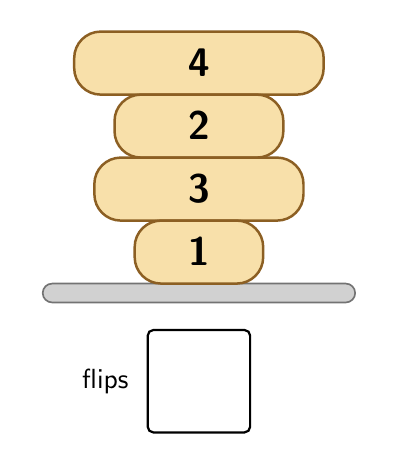
\begin{tikzpicture}
\useasboundingbox (-2.175,-1.940) rectangle (2.175,3.250);
\draw[platedraw, platefill, rounded corners=0.120cm] (-1.984,-0.240) rectangle (1.984,0);
\fill[cakefill] [rounded corners=0.336cm] (-1.584,2.400) rectangle (1.584,3.200);
\draw[cakedraw] [rounded corners=0.336cm] (-1.584,2.400) rectangle (1.584,3.200);
\node[font=\Large\bfseries, inner sep=0pt] at (0.000,2.800) {4};
\fill[cakefill] [rounded corners=0.336cm] (-1.072,1.600) rectangle (1.072,2.400);
\draw[cakedraw] [rounded corners=0.336cm] (-1.072,1.600) rectangle (1.072,2.400);
\node[font=\Large\bfseries, inner sep=0pt] at (0.000,2.000) {2};
\fill[cakefill] [rounded corners=0.336cm] (-1.328,0.800) rectangle (1.328,1.600);
\draw[cakedraw] [rounded corners=0.336cm] (-1.328,0.800) rectangle (1.328,1.600);
\node[font=\Large\bfseries, inner sep=0pt] at (0.000,1.200) {3};
\fill[cakefill] [rounded corners=0.336cm] (-0.816,0.000) rectangle (0.816,0.800);
\draw[cakedraw] [rounded corners=0.336cm] (-0.816,0.000) rectangle (0.816,0.800);
\node[font=\Large\bfseries, inner sep=0pt] at (0.000,0.400) {1};
\node[anchor=east, font=\normalsize] at (-0.770,-1.240) {flips};
\draw[thick, rounded corners=2pt] (-0.650,-1.890) rectangle (0.650,-0.590);
\end{tikzpicture}\hfill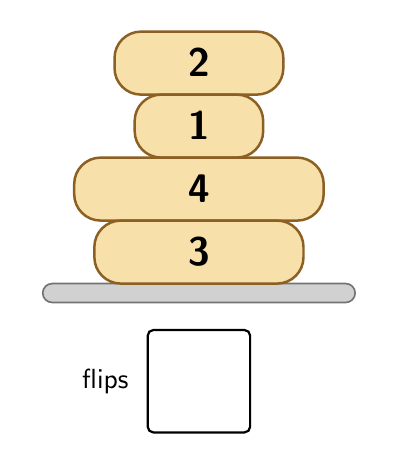
\begin{tikzpicture}
\useasboundingbox (-2.175,-1.940) rectangle (2.175,3.250);
\draw[platedraw, platefill, rounded corners=0.120cm] (-1.984,-0.240) rectangle (1.984,0);
\fill[cakefill] [rounded corners=0.336cm] (-1.072,2.400) rectangle (1.072,3.200);
\draw[cakedraw] [rounded corners=0.336cm] (-1.072,2.400) rectangle (1.072,3.200);
\node[font=\Large\bfseries, inner sep=0pt] at (0.000,2.800) {2};
\fill[cakefill] [rounded corners=0.336cm] (-0.816,1.600) rectangle (0.816,2.400);
\draw[cakedraw] [rounded corners=0.336cm] (-0.816,1.600) rectangle (0.816,2.400);
\node[font=\Large\bfseries, inner sep=0pt] at (0.000,2.000) {1};
\fill[cakefill] [rounded corners=0.336cm] (-1.584,0.800) rectangle (1.584,1.600);
\draw[cakedraw] [rounded corners=0.336cm] (-1.584,0.800) rectangle (1.584,1.600);
\node[font=\Large\bfseries, inner sep=0pt] at (0.000,1.200) {4};
\fill[cakefill] [rounded corners=0.336cm] (-1.328,0.000) rectangle (1.328,0.800);
\draw[cakedraw] [rounded corners=0.336cm] (-1.328,0.000) rectangle (1.328,0.800);
\node[font=\Large\bfseries, inner sep=0pt] at (0.000,0.400) {3};
\node[anchor=east, font=\normalsize] at (-0.770,-1.240) {flips};
\draw[thick, rounded corners=2pt] (-0.650,-1.890) rectangle (0.650,-0.590);
\end{tikzpicture}\hfill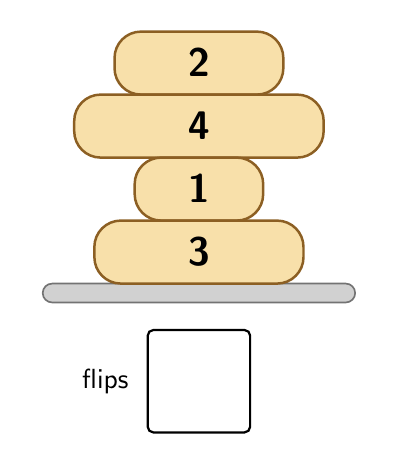
\begin{tikzpicture}
\useasboundingbox (-2.175,-1.940) rectangle (2.175,3.250);
\draw[platedraw, platefill, rounded corners=0.120cm] (-1.984,-0.240) rectangle (1.984,0);
\fill[cakefill] [rounded corners=0.336cm] (-1.072,2.400) rectangle (1.072,3.200);
\draw[cakedraw] [rounded corners=0.336cm] (-1.072,2.400) rectangle (1.072,3.200);
\node[font=\Large\bfseries, inner sep=0pt] at (0.000,2.800) {2};
\fill[cakefill] [rounded corners=0.336cm] (-1.584,1.600) rectangle (1.584,2.400);
\draw[cakedraw] [rounded corners=0.336cm] (-1.584,1.600) rectangle (1.584,2.400);
\node[font=\Large\bfseries, inner sep=0pt] at (0.000,2.000) {4};
\fill[cakefill] [rounded corners=0.336cm] (-0.816,0.800) rectangle (0.816,1.600);
\draw[cakedraw] [rounded corners=0.336cm] (-0.816,0.800) rectangle (0.816,1.600);
\node[font=\Large\bfseries, inner sep=0pt] at (0.000,1.200) {1};
\fill[cakefill] [rounded corners=0.336cm] (-1.328,0.000) rectangle (1.328,0.800);
\draw[cakedraw] [rounded corners=0.336cm] (-1.328,0.000) rectangle (1.328,0.800);
\node[font=\Large\bfseries, inner sep=0pt] at (0.000,0.400) {3};
\node[anchor=east, font=\normalsize] at (-0.770,-1.240) {flips};
\draw[thick, rounded corners=2pt] (-0.650,-1.890) rectangle (0.650,-0.590);
\end{tikzpicture}\hfill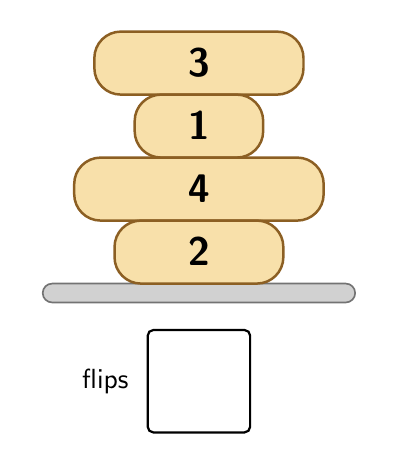
\begin{tikzpicture}
\useasboundingbox (-2.175,-1.940) rectangle (2.175,3.250);
\draw[platedraw, platefill, rounded corners=0.120cm] (-1.984,-0.240) rectangle (1.984,0);
\fill[cakefill] [rounded corners=0.336cm] (-1.328,2.400) rectangle (1.328,3.200);
\draw[cakedraw] [rounded corners=0.336cm] (-1.328,2.400) rectangle (1.328,3.200);
\node[font=\Large\bfseries, inner sep=0pt] at (0.000,2.800) {3};
\fill[cakefill] [rounded corners=0.336cm] (-0.816,1.600) rectangle (0.816,2.400);
\draw[cakedraw] [rounded corners=0.336cm] (-0.816,1.600) rectangle (0.816,2.400);
\node[font=\Large\bfseries, inner sep=0pt] at (0.000,2.000) {1};
\fill[cakefill] [rounded corners=0.336cm] (-1.584,0.800) rectangle (1.584,1.600);
\draw[cakedraw] [rounded corners=0.336cm] (-1.584,0.800) rectangle (1.584,1.600);
\node[font=\Large\bfseries, inner sep=0pt] at (0.000,1.200) {4};
\fill[cakefill] [rounded corners=0.336cm] (-1.072,0.000) rectangle (1.072,0.800);
\draw[cakedraw] [rounded corners=0.336cm] (-1.072,0.000) rectangle (1.072,0.800);
\node[font=\Large\bfseries, inner sep=0pt] at (0.000,0.400) {2};
\node[anchor=east, font=\normalsize] at (-0.770,-1.240) {flips};
\draw[thick, rounded corners=2pt] (-0.650,-1.890) rectangle (0.650,-0.590);
\end{tikzpicture}\hfill}

\newpage
\problem{5}Each pancake has a dark side. Sort each stack so every dark side ends facing down, with as few flips as you can.
\par\smallskip\begin{center}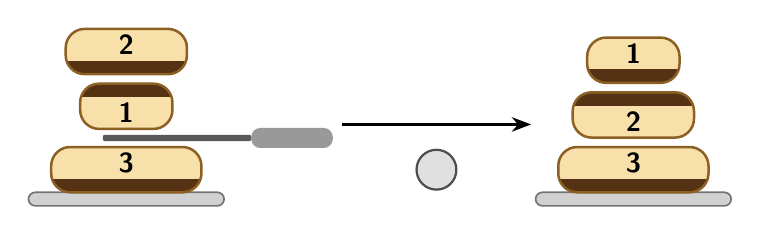
\begin{tikzpicture}
\draw[platedraw, platefill, rounded corners=0.086cm] (-1.242,-0.172) rectangle (1.242,0);
\fill[cakefill] [rounded corners=0.241cm] (-0.770,1.500) rectangle (0.770,2.075);
\begin{scope}
\clip [rounded corners=0.241cm] (-0.770,1.500) rectangle (0.770,2.075);
\fill[burnt] (-0.770,1.500) rectangle (0.770,1.672);
\end{scope}
\draw[cakedraw] [rounded corners=0.241cm] (-0.770,1.500) rectangle (0.770,2.075);
\node[font=\normalsize\bfseries, inner sep=0pt] at (0.000,1.874) {2};
\fill[cakefill] [rounded corners=0.241cm] (-0.586,0.805) rectangle (0.586,1.380);
\begin{scope}
\clip [rounded corners=0.241cm] (-0.586,0.805) rectangle (0.586,1.380);
\fill[burnt] (-0.586,1.208) rectangle (0.586,1.380);
\end{scope}
\draw[cakedraw] [rounded corners=0.241cm] (-0.586,0.805) rectangle (0.586,1.380);
\node[font=\normalsize\bfseries, inner sep=0pt] at (0.000,1.006) {1};
\fill[cakefill] [rounded corners=0.241cm] (-0.954,0.000) rectangle (0.954,0.575);
\begin{scope}
\clip [rounded corners=0.241cm] (-0.954,0.000) rectangle (0.954,0.575);
\fill[burnt] (-0.954,0.000) rectangle (0.954,0.172);
\end{scope}
\draw[cakedraw] [rounded corners=0.241cm] (-0.954,0.000) rectangle (0.954,0.575);
\node[font=\normalsize\bfseries, inner sep=0pt] at (0.000,0.374) {3};
\fill[spatula, rounded corners=0.5pt] (-0.299,0.650) rectangle (1.587,0.730);
\fill[handle, rounded corners=0.114cm] (1.587,0.563) rectangle (2.622,0.817);
\draw[-{Stealth[length=7pt]}, thick] (2.737,0.862) -- (5.141,0.862);
\draw[tokdraw, tokfill] (3.939,0.287) circle (0.253);
\draw[platedraw, platefill, rounded corners=0.086cm] (5.198,-0.172) rectangle (7.682,0);
\fill[cakefill] [rounded corners=0.241cm] (5.853,1.390) rectangle (7.026,1.965);
\begin{scope}
\clip [rounded corners=0.241cm] (5.853,1.390) rectangle (7.026,1.965);
\fill[burnt] (5.853,1.390) rectangle (7.026,1.562);
\end{scope}
\draw[cakedraw] [rounded corners=0.241cm] (5.853,1.390) rectangle (7.026,1.965);
\node[font=\normalsize\bfseries, inner sep=0pt] at (6.440,1.764) {1};
\fill[cakefill] [rounded corners=0.241cm] (5.669,0.695) rectangle (7.210,1.270);
\begin{scope}
\clip [rounded corners=0.241cm] (5.669,0.695) rectangle (7.210,1.270);
\fill[burnt] (5.669,1.098) rectangle (7.210,1.270);
\end{scope}
\draw[cakedraw] [rounded corners=0.241cm] (5.669,0.695) rectangle (7.210,1.270);
\node[font=\normalsize\bfseries, inner sep=0pt] at (6.440,0.896) {2};
\fill[cakefill] [rounded corners=0.241cm] (5.486,0.000) rectangle (7.394,0.575);
\begin{scope}
\clip [rounded corners=0.241cm] (5.486,0.000) rectangle (7.394,0.575);
\fill[burnt] (5.486,0.000) rectangle (7.394,0.172);
\end{scope}
\draw[cakedraw] [rounded corners=0.241cm] (5.486,0.000) rectangle (7.394,0.575);
\node[font=\normalsize\bfseries, inner sep=0pt] at (6.440,0.374) {3};
\end{tikzpicture}\end{center}
\par\vspace{0.6cm}
\noindent\makebox[\linewidth][s]{\hfill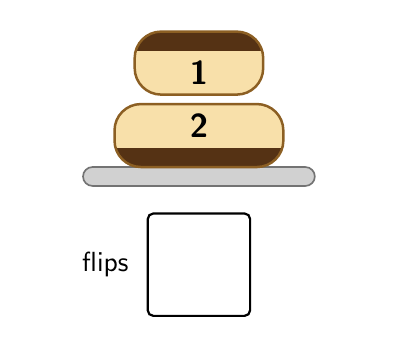
\begin{tikzpicture}
\useasboundingbox (-2.175,-1.940) rectangle (2.175,1.770);
\draw[platedraw, platefill, rounded corners=0.120cm] (-1.472,-0.240) rectangle (1.472,0);
\fill[cakefill] [rounded corners=0.336cm] (-0.816,0.920) rectangle (0.816,1.720);
\begin{scope}
\clip [rounded corners=0.336cm] (-0.816,0.920) rectangle (0.816,1.720);
\fill[burnt] (-0.816,1.480) rectangle (0.816,1.720);
\end{scope}
\draw[cakedraw] [rounded corners=0.336cm] (-0.816,0.920) rectangle (0.816,1.720);
\node[font=\large\bfseries, inner sep=0pt] at (0.000,1.200) {1};
\fill[cakefill] [rounded corners=0.336cm] (-1.072,0.000) rectangle (1.072,0.800);
\begin{scope}
\clip [rounded corners=0.336cm] (-1.072,0.000) rectangle (1.072,0.800);
\fill[burnt] (-1.072,0.000) rectangle (1.072,0.240);
\end{scope}
\draw[cakedraw] [rounded corners=0.336cm] (-1.072,0.000) rectangle (1.072,0.800);
\node[font=\large\bfseries, inner sep=0pt] at (0.000,0.520) {2};
\node[anchor=east, font=\normalsize] at (-0.770,-1.240) {flips};
\draw[thick, rounded corners=2pt] (-0.650,-1.890) rectangle (0.650,-0.590);
\end{tikzpicture}\hfill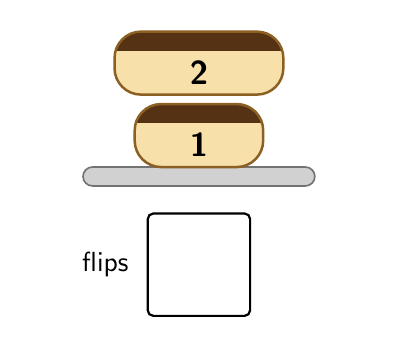
\begin{tikzpicture}
\useasboundingbox (-2.175,-1.940) rectangle (2.175,1.770);
\draw[platedraw, platefill, rounded corners=0.120cm] (-1.472,-0.240) rectangle (1.472,0);
\fill[cakefill] [rounded corners=0.336cm] (-1.072,0.920) rectangle (1.072,1.720);
\begin{scope}
\clip [rounded corners=0.336cm] (-1.072,0.920) rectangle (1.072,1.720);
\fill[burnt] (-1.072,1.480) rectangle (1.072,1.720);
\end{scope}
\draw[cakedraw] [rounded corners=0.336cm] (-1.072,0.920) rectangle (1.072,1.720);
\node[font=\large\bfseries, inner sep=0pt] at (0.000,1.200) {2};
\fill[cakefill] [rounded corners=0.336cm] (-0.816,0.000) rectangle (0.816,0.800);
\begin{scope}
\clip [rounded corners=0.336cm] (-0.816,0.000) rectangle (0.816,0.800);
\fill[burnt] (-0.816,0.560) rectangle (0.816,0.800);
\end{scope}
\draw[cakedraw] [rounded corners=0.336cm] (-0.816,0.000) rectangle (0.816,0.800);
\node[font=\large\bfseries, inner sep=0pt] at (0.000,0.280) {1};
\node[anchor=east, font=\normalsize] at (-0.770,-1.240) {flips};
\draw[thick, rounded corners=2pt] (-0.650,-1.890) rectangle (0.650,-0.590);
\end{tikzpicture}\hfill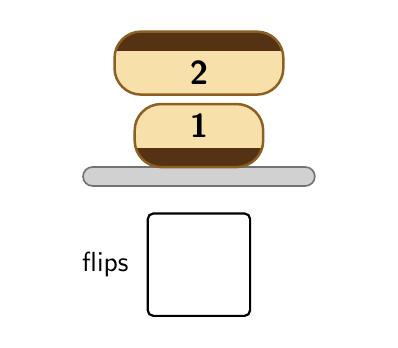
\begin{tikzpicture}
\useasboundingbox (-2.175,-1.940) rectangle (2.175,1.770);
\draw[platedraw, platefill, rounded corners=0.120cm] (-1.472,-0.240) rectangle (1.472,0);
\fill[cakefill] [rounded corners=0.336cm] (-1.072,0.920) rectangle (1.072,1.720);
\begin{scope}
\clip [rounded corners=0.336cm] (-1.072,0.920) rectangle (1.072,1.720);
\fill[burnt] (-1.072,1.480) rectangle (1.072,1.720);
\end{scope}
\draw[cakedraw] [rounded corners=0.336cm] (-1.072,0.920) rectangle (1.072,1.720);
\node[font=\large\bfseries, inner sep=0pt] at (0.000,1.200) {2};
\fill[cakefill] [rounded corners=0.336cm] (-0.816,0.000) rectangle (0.816,0.800);
\begin{scope}
\clip [rounded corners=0.336cm] (-0.816,0.000) rectangle (0.816,0.800);
\fill[burnt] (-0.816,0.000) rectangle (0.816,0.240);
\end{scope}
\draw[cakedraw] [rounded corners=0.336cm] (-0.816,0.000) rectangle (0.816,0.800);
\node[font=\large\bfseries, inner sep=0pt] at (0.000,0.520) {1};
\node[anchor=east, font=\normalsize] at (-0.770,-1.240) {flips};
\draw[thick, rounded corners=2pt] (-0.650,-1.890) rectangle (0.650,-0.590);
\end{tikzpicture}\hfill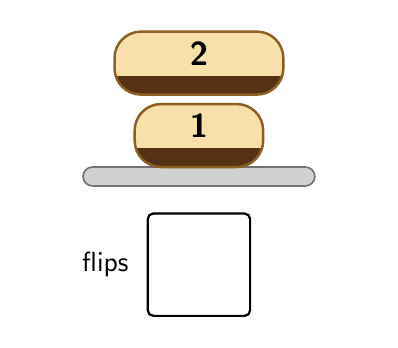
\begin{tikzpicture}
\useasboundingbox (-2.175,-1.940) rectangle (2.175,1.770);
\draw[platedraw, platefill, rounded corners=0.120cm] (-1.472,-0.240) rectangle (1.472,0);
\fill[cakefill] [rounded corners=0.336cm] (-1.072,0.920) rectangle (1.072,1.720);
\begin{scope}
\clip [rounded corners=0.336cm] (-1.072,0.920) rectangle (1.072,1.720);
\fill[burnt] (-1.072,0.920) rectangle (1.072,1.160);
\end{scope}
\draw[cakedraw] [rounded corners=0.336cm] (-1.072,0.920) rectangle (1.072,1.720);
\node[font=\large\bfseries, inner sep=0pt] at (0.000,1.440) {2};
\fill[cakefill] [rounded corners=0.336cm] (-0.816,0.000) rectangle (0.816,0.800);
\begin{scope}
\clip [rounded corners=0.336cm] (-0.816,0.000) rectangle (0.816,0.800);
\fill[burnt] (-0.816,0.000) rectangle (0.816,0.240);
\end{scope}
\draw[cakedraw] [rounded corners=0.336cm] (-0.816,0.000) rectangle (0.816,0.800);
\node[font=\large\bfseries, inner sep=0pt] at (0.000,0.520) {1};
\node[anchor=east, font=\normalsize] at (-0.770,-1.240) {flips};
\draw[thick, rounded corners=2pt] (-0.650,-1.890) rectangle (0.650,-0.590);
\end{tikzpicture}\hfill}

\par\vspace{1.4cm}
\problem{6}Find the stack of pancakes 1 and 2 that needs the most flips. Draw it with its dark sides.
\par\bigskip
\noindent\makebox[\linewidth][s]{\hfill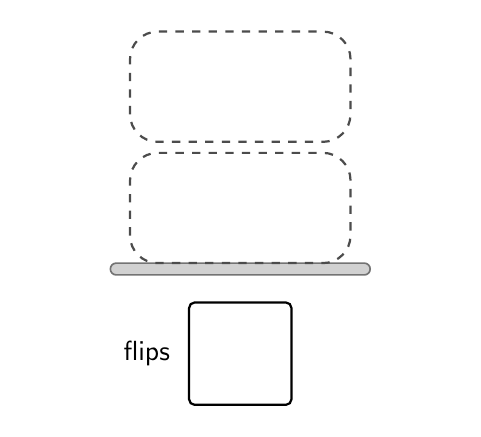
\begin{tikzpicture}
\useasboundingbox (-2.700,-1.850) rectangle (2.700,2.990);
\draw[platedraw, platefill, rounded corners=0.075cm] (-1.650,-0.150) rectangle (1.650,0);
\draw[slot, rounded corners=0.350cm] (-1.400,1.540) rectangle (1.400,2.940);
\draw[slot, rounded corners=0.350cm] (-1.400,0.000) rectangle (1.400,1.400);
\node[anchor=east, font=\normalsize] at (-0.770,-1.150) {flips};
\draw[thick, rounded corners=2pt] (-0.650,-1.800) rectangle (0.650,-0.500);
\end{tikzpicture}\hfill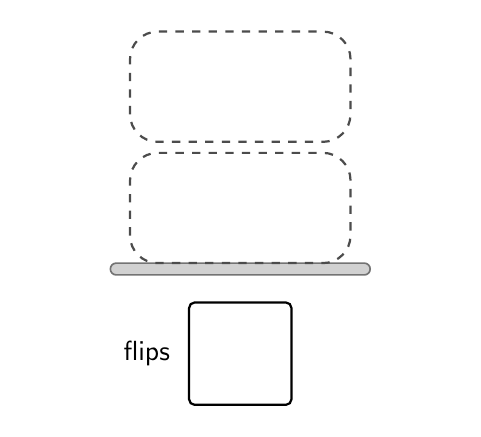
\begin{tikzpicture}
\useasboundingbox (-2.700,-1.850) rectangle (2.700,2.990);
\draw[platedraw, platefill, rounded corners=0.075cm] (-1.650,-0.150) rectangle (1.650,0);
\draw[slot, rounded corners=0.350cm] (-1.400,1.540) rectangle (1.400,2.940);
\draw[slot, rounded corners=0.350cm] (-1.400,0.000) rectangle (1.400,1.400);
\node[anchor=east, font=\normalsize] at (-0.770,-1.150) {flips};
\draw[thick, rounded corners=2pt] (-0.650,-1.800) rectangle (0.650,-0.500);
\end{tikzpicture}\hfill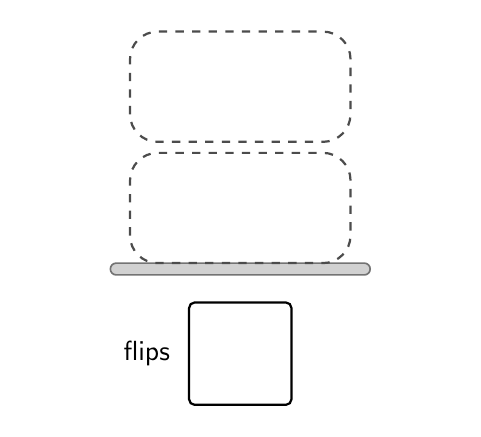
\begin{tikzpicture}
\useasboundingbox (-2.700,-1.850) rectangle (2.700,2.990);
\draw[platedraw, platefill, rounded corners=0.075cm] (-1.650,-0.150) rectangle (1.650,0);
\draw[slot, rounded corners=0.350cm] (-1.400,1.540) rectangle (1.400,2.940);
\draw[slot, rounded corners=0.350cm] (-1.400,0.000) rectangle (1.400,1.400);
\node[anchor=east, font=\normalsize] at (-0.770,-1.150) {flips};
\draw[thick, rounded corners=2pt] (-0.650,-1.800) rectangle (0.650,-0.500);
\end{tikzpicture}\hfill}

\end{document}
